\chapter{Riemannian manifolds}

\setcounter{section}{1}
\setcounter{subsection}{0}

\subsection{}\label{chap3:3.1.1}

\begin{defi*}
Let\pageoriginale $M$ be a manifold. An element
$g\in\mathscr{L}^{2}(M)$ is said to 
define a {\em Riemannian structure} (or {\em simply} r.s.) on $M$, if
for every $m$ in $M$, $g_{m}\in\mathscr{L}^{2}(T_{m}(M))$ defines a
euclidean structure on $T_{m}(M)$ (see (\ref{chap0:0.3.3})). A manifold $M$
with an r.s.\@ is called a {\em Riemannian manifold} (or {\em simply}
r.m.). {\em By} $(M,g)$ we denote the r.m. $M$ with the r.s.g.\@
\end{defi*}

\subsection{}\label{chap3:3.1.2}

\begin{examples*}
1.~As a first example of an r.m. we endow $\mathbb{R}^{d}$ with the
r.s., denoted by $\epsilon$; defined by the equation
$$
\epsilon(X,Y)=(\zeta\circ X)\cdot (\zeta\circ Y),\forall X,
Y\in\mathscr{C}(\mathbb{R}^{d}) 
$$
where denotes the usual scalar product on $\mathbb{R}^{d}$.
\end{examples*}

\setcounter{subsection}{2}
\subsection{}\label{chap3:3.1.3}
Let $(M,g)$ be any r.m., and let $U$ be an open subset of $M$. Then
the restriction of $g$ to $U$ defines an r.s.\@ on $U$, denoted
sometimes by $g|U$. Whenever we consider an open subset of an r.m. as
an r.m. it is the structure above we have in mind.

\subsection{}\label{chap3:3.1.4}

\begin{remarks*}
Given an r.s.\@ $g$ on $M$, we have, for every $m$ of $M$, a positive
definite symmetric bilinear form $g_{m}$ on $T_{m}(M)$ which depends
differentiably on $m$, i.e. the map
$$
g:m\to g_{m}
$$
belongs to $D(M,L^{2}(T(M))$. The converse of this statement follows
from (\ref{chap0:0.2.3}).
\end{remarks*}

The above examples make it possible to define an r.s.\@ on every
manifold $M$. To\pageoriginale see this, let $(U_{i},r_{i})$ be a
family of charts of $M$ such that the $U_{i}$ cover $M$ and let
$\{\varphi_{i}\}$ be a partition of unity (see (\ref{chap0:sec1}))
subordinate to the covering $\{U_{i}\}$. By (\ref{chap3:3.1.3}) on
each $U_{i}$ we have an r.s.\@ namely $r^{\ast}_{i}(\epsilon_{i})$ where
$\epsilon_{i}=\epsilon|r_{i}(U_{i})$ is the restriction of $\epsilon$
to $r_{i}(U_{i})$. Now let us extend the form
$\varphi_{i}r^{\ast}_{i}(\epsilon_{i})$ to the whole of $M$ by
defining it to be zero outside $U_{i}$. Then
$$
\varphi_{i}\cdot r^{\ast}_{i}(\epsilon_{i})\in D(M,L^{2}(T(M)),
$$
and set
$$
h=\sum_{i}\varphi_{i}r^{\ast}_{i}(\epsilon_{i}).
$$
Then we have for every $X$, $Y$ in $\mathscr{C}(M)$, and $m$ in $M$,
\begin{align*}
h(X,Y) &= \sum_{i}\varphi_{i}\cdot r^{\ast}_{i}(\epsilon_{i})(X,Y)=\\
&= \sum_{i}\varphi_{i}r^{\ast}_{i}(\epsilon_{i})(Y,X)\quad\text{since
  $\epsilon$ is symmetric}\\
&= h(Y,X),
\end{align*}
and
\begin{align*}
h(X,X)(m) &= \sum_{i}\varphi_{i}(m)r^{\ast}_{i}(\epsilon_{i})(X,X)=\\
&= \sum_{i}\varphi_{i}(m)\epsilon(r^{T}_{i}(X),r^{T}_{i}(X))(m).
\end{align*}
Since $\sum \varphi_{i}(m)=1$ there is an $i_{0}$ such that
$\varphi_{i_{0}}(m)\neq 0$ and since $\varphi_{i}\geq 0$ and $r_{i}$
are diffeomorphisms we have
$$
\sum_{i}\varphi_{i}(m)\cdot \epsilon(r^{T}_{i}X(m),r^{T}_{i}X(m))\geq
\varphi_{i_{0}}(m)\cdot \epsilon(r^{T}_{i_{0}}X(m),r^{T}_{i_{0}}X(m))>0,
$$
if $X(m)\neq 0$. Hence \pageoriginale $h$ is symmetric and positive
definite and clearly bilinear. Hence every manifold admits an r.s.

Given two vectors $x$ and $y$ such that $p(x)=p(y)$ then $g(x,y)$ is
defined and we call $g(x,y)$ the {\em scalar product} of $x$ and
$y$. Associated to this scalar product there is a {\em norm},
$||\;||$, on $T(M)$; namely
\begin{equation*}
||x||=(g(x,x))^{\frac{1}{2}}.\tag{3.1.5}\label{chap3:3.1.5}
\end{equation*}

\setcounter{subsection}{5}
\subsection{}\label{chap3:3.1.6}
We denote $g(x,x)=||x||^{2}$ by $E(x)$ and note that $E:T(M)\to
\mathbb{R}$ is differentiable and $||\;||$ is continuous ($E$ stands 
for {\em energy}).

\subsection{}\label{chap3:3.1.7}
On the tangent space $T_{m}(M)$ of $M$ at $m$ the topology induced by
$T(M)$ and that induced by the norm $||\;||$ are the same. 

\setcounter{subsection}{7}

\subsection{}\label{chap3:3.1.8} %%%

\begin{lemma*}
$\forall x\in T(M)$ and $z\in V_{x}$ we have
$$
z(E)=2g(x,\xi(z)).
$$
\end{lemma*}

\begin{proof}
Let
$$
i:T_{p(x)}(M)\to T(M)
$$
be the canonical injection. Then
$$
z(E)=(i^{T})^{-1}(z)(E\circ i)
$$
where $E\circ i$ is the quadratic form on $T_{p(x)}(M)$ associated to
$g_{p(x)}$. Then (see \cite{36} and (\ref{chap0:0.4.11})):
$$
z(E)=2g(x,\zeta((i^{T})^{-1})(z))=2g(x,\xi(z)).
$$
\end{proof}

\subsection{}\label{chap3:3.1.9}

\begin{defi*}
We \pageoriginale say that an r.m. $(M\cdot g)$ is {\em isometric} to
an r.m. $(N,h)$ if there exists an $f\in D(M,N)$ such that
\begin{itemize}
\item[i)] $f$ is a diffeomorphism,

\item[ii)] $f^{\ast}h=g$.
\end{itemize}
Then $f$ is called an {\em isometry} between $(M,g)$ and $(N,h)$. We
say that $(M,g)$ is {\em locally isometric} to $(N,h)$ if, $\forall
m\in M$, there exists an open neighbourhood $U$ of $m$ in $M$ and a
map $f\in D(U,N)$ such that:
\begin{itemize}
\item[i)] $f(U)$ is open in $N$,

\item[ii)] $f$ is an isometry between $(U,g|U)$ and $(f(U),h|f(U))$.
\end{itemize}
\end{defi*}

\subsection{Orthogonal vector fields.}\label{chap3:3.1.10}

Let us consider $(\mathbb{R}^{d},\epsilon)$. Then the canonical basis
$\dfrac{\partial}{\partial u^{1}},\ldots,\dfrac{\partial}{\partial
  u^{d}}$ has the following two properties:
\begin{itemize}
\item[i)] orthogonality: $\epsilon\left(\dfrac{\partial}{\partial
  u^{i}},\dfrac{\partial}{\partial u^{j}}\right)=0$ if $i\neq j$,

\item[ii)] commutativity: $\left[\dfrac{\partial}{\partial
    u^{i}},\dfrac{\partial}{\partial u^{j}}\right]=0$. 
\end{itemize}

\setcounter{subsection}{10}
\subsection{}\label{chap3:3.1.11}
In the case of a manifold $(M,g)$, locally, we can select an
orthonormal basis for $\mathscr{C}(M)$. To see this let $(U,r)$ be a
chart of $M$ and let $X_{1},\ldots,X_{d}$ be a basis of
$\mathscr{C}(U)$, say for example the one got by pulling back the
canonical basis on $r(U)$. The define $Y'_{i}$ and $Y_{i}$ inductively
by setting $Y'_{1}=Y_{1}=\dfrac{X_{1}}{||X_{1}||}$, \pageoriginale
division by $||X_{1}||$ is possible since $X_{1}$ is a basis element
and hence never zero,
\begin{align*}
Y'_{i} &= X_{i}-\sum^{i-1}_{k=1}g(X_{i},Y_{k})Y_{k}\\
Y_{i} &= \frac{Y'_{i}}{||Y'_{i}||},\quad\text{($Y'_{i}$ is never zero
  since $\{X_{i}\}$ is a basis)}.
\end{align*}
Then $Y_{1},\ldots,Y_{d}$ is an orthonormal basis of $\mathscr{C}(U)$.

By pulling back the canonical basis on $\mathscr{C}(r(U))$ we get a
commutative basis of $\mathscr{C}(U)$. But, in general, there is not
any local orthonormal basis of $\mathscr{C}(M)$ which is also
commutative. For, relative to $(U,r)$ a chart of $M$, let
$Y_{1},\ldots,Y_{d}$ be an orthonormal basis of $\mathscr{C}(U)$ such
that
$$
[Y_{i},Y_{j}]=0.
$$
Then by Frobenius's theorem there exists a local system of coordinates
$y^{1},\ldots,y^{d}$ such that
$$
Y_{i}=\frac{\partial}{\partial y^{i}} \; i=1,\ldots,d.
$$
Then the map
$$
f:m\to (y^{1}(m),\ldots,y^{d}(m))
$$
gives a local isometry between $U$ and $\mathbb{R}^{d}$. For clearly
$f$ is a diffeomorphism, and
\begin{align*}
(f^{\ast}\epsilon)(Y_{i},Y_{j})
  &=\epsilon(f^{T}(Y_{i}),f^{T}(Y_{j}))\\
&= \epsilon\left(\frac{\partial}{\partial
    y^{i}},\frac{\partial}{\partial y^{j}}\right)=\delta_{ij}=g(Y_{i},Y_{j}),
\end{align*}
and \pageoriginale hence $g=f^{\ast}\epsilon$. But in general r.m.'s
are not locally isometric to $\mathbb{R}^{d}$ (see (\ref{chap5:5.5.2}) and
(\ref{chap2:2.5.4})). 

\setcounter{section}{1}
\section{Examples}\label{chap3:sec2}

\subsection{}\label{chap3:3.2.1}
Suppose that $(M,g)$ is an r.m. and $N$ any manifold such that there
exists a map $f\in D(N,M)$:
$$
f:N\to M
$$
such that $f^{T}_{n}$ is injective for every $n\in N$. Then
$f^{\ast}g\in \mathscr{L}^{2}(N)$ and $(f^{\ast}g)_{n}$ is symmetric
on $T_{n}(N)$. Moreover for $x\in T_{n}(N)$ if $(f^{\ast}g)(x,x)=0$
then $0=(f^{\ast}g)(x,x)=g(f^{T}_{n}(x)$, $f^{T}_{n}(x))$ and since
$g$ is positive definite we have $f^{T}_{n}(x)=0$. But $f^{T}_{n}$ is
injective and hence $x=0$. Hence $f^{\ast}g$ is positive
definite. Therefore $f^{\ast}g$ defines an r.s.\@ on $N$. We apply this
remark to the following cases.
\begin{enumerate}
\renewcommand{\theenumi}{\Alph{enumi}}
\renewcommand{\labelenumi}{\theenumi)}
\item Let $N$ be an sub-manifold of $(M,g)$. Then the injection
$$
i:N\to M
$$
has the properties stated above for $f$ and hence we have an r.s.,
called the {\em induced r.s.,} on $N$. We denote it by $(g|N)$.

\quad 
The study, initiated by Gauss, of surfaces $S$ in $\mathbb{R}^{3}$,
i.e. of two dimensional sub-manifolds $S$ with the induced structure
was the starting point for Riemann's original investigations on this
subject. On the other hand, the theorem of Nash (\cite{34}) states
that if $(M,g)$ is a connected r.m. then there exists an integer $d'$
and a diffeomorphism $f$ between $M$ and a sub-manifold $N$ of
$\mathbb{R}^{d'}$ such that $f$ is an isometry between $(M,g)$ and
$(N,\epsilon|N)$.

\item Let \pageoriginale us consider the sphere $\mathbb{S}^{d}$:
$$
\mathbb{S}^{d}=\{x\in\mathbb{R}^{d+1}|x\cdot x=1\}\subset
(\mathbb{R}^{d+1},\epsilon).
$$
Then $\epsilon|\mathbb{S}^{d}$ is called the canonical r.s.\@ on
$\mathbb{S}^{d}$. Let us note that any element of the orthogonal group
of $\mathbb{R}^{d+1}$ induces an isometry on
$(\mathbb{S}^{d},\epsilon|\mathbb{S}^{d})$.

\item Suppose that $(N,h)$ is an r.m., $M$ is any manifold and $f\in
  D(M,N)$ is a {\em covering map} i.e. a map such that to each point
  $n$ of $N$ there is a neighbourhood $U$ such that $f$ restricted to
  each connected component of $f^{-1}(U)$ is a homeomorphism between
  that component and $U$. Then $f^{\ast}h$ defines an r.s.\@ on $M$ and
  this situation is described by saying that $f$ is a {\em Riemannian
    covering}. Note that, in this case, $(M,f^{\ast}g)$ and $(N,h)$
  are locally isometric. 
\end{enumerate}

\subsection{}\label{chap3:3.2.2}) 
Now let us suppose that $(M,g)$
  is an r.m. and that $G$ is a discrete group of isometries of $(M,g)$
  without fixed points. If the quotient $M/G$ is a manifold, then the
  canonical map $p$:
$$
p:M\to M/G
$$
is a covering map, and there is a unique r.s.\@ on $M/G$, denoted by
$g/G$, for which $p:M\to M/G$ is a Riemannian covering.

\quad 
To see this, let $n\in M/G$ and let $m\in p^{-1}(n)$. Then since $p$
is a covering map it is a local diffeomorphism, and we naturally
define
$$
h_{n}=(p^{-1})^{\ast}g_{m}
$$
and $h_{n}$ defines a euclidean structure on $T_{m}(M)$. Since $G$ is
a group \pageoriginale of isometries it follows that $h_{n}$ is
independent of the $m$ chosen. Thus we have a map
$$
h:n\to h_{n}
$$
of $N$ into $L^{2}(T(M/G))$. Furthermore since $p$ is a local
diffeomorphism, and since the differentiability is a local property it
follows that $h$ is differentiable. Hence there is an r.s.\@ with the
above properties.

\begin{enumerate}
\item[D)] Let us note two particular cases.
\begin{enumerate}
\renewcommand{\theenumii}{\arabic{enumii}}
\renewcommand{\labelenumii}{\theenumii.}
\item For $(M,g)$ take $(\mathbb{S}^{d},\epsilon|\mathbb{S}^{d})$ and
  for $G$ take the group generated by the antipodal map of
  $\mathbb{S}^{d}$, i.e. the one induced on $\mathbb{S}^{d}$ by the
  map $-\id_{\mathbb{R}^{d+1}}$ of $\mathbb{R}^{d+1}$. Then
  $\mathbb{S}^{d}/G$ is the real projective space
  ($P^{d}(\mathbb{R}))$, can).

\item For $(M,g)$ take $(\mathbb{R}^{d},\epsilon)$ and for $G$ take a
  discrete subgroup of the group of all translations of
  $\mathbb{R}^{d}$ such that the rank of $G$ is $d$. Then the {\em
    torus} $\mathbb{R}^{d}/G$ considered as an r.m.\@ with the r.s.\@
  $\mathbb{R}^{d}/G$ is called a {\em flat torus} and denoted by
  $(\mathbb{R}^{d}/G,\epsilon/G)$.  
\end{enumerate}
\end{enumerate}

\section{Symmetric pairs}\label{chap3:sec3}

\subsection{}\label{chap3:3.3.1}

Let $G$ be a Lie group and let $\lambda(s)$ and $\rho(s)$ denote the
left and the right multiplications by $s\in G$. Further let
$\underbar{G}$ be the Lie algebra of $G$ and $\exp:\underbar{G}\to G$
the associated exponential map. Let $X\in\underbar{G}$; then the
vector field defined by the one parameter group
$$
\lambda(\exp(tX)),t\in\mathbb{R}
$$
is the right invariant vector field whose value at $e$ (the neutral
element of $G$) is $X$. To see this we have only to compute the speed
of the \pageoriginale curve $t\to (\exp(tX))g$, at $t=0$.

But
$$
(\exp(tX))g=\rho(g)(\exp(tX)),
$$
so that
$$
(\rho(g)\circ (\exp(tX)))'(0)=(\rho(g))^{T}(\exp(tX))'(0)
$$
and by the definition of the $\exp$ map
$$
(\exp(tX))'(0)=X.
$$
Hence the result.

\setcounter{definition}{1}

\subsection{}\label{chap3:3.3.2}

\begin{defi*}
{\em A symmetric pair} $(G,H,\sigma)$ consists of
\begin{itemize}
\item[1)] a connected Lie group $G$

\item[2)] a compact subgroup $H$ of $G$ and

\item[3)] an involutive automorphism $\sigma$ of $G$ such that
$$
\sum_{0}\subset H\subset \sum
$$
where $\sum$ is the subgroup of elements in $G$ fixed by $\sigma$, and
$\sum_{0}$ is the connected component of the identity, $e$ of $\sum$.
\end{itemize}

When no confusion is possible, we shall speak of the symmetric pair
$(G,H)$ without any reference to $\sigma$.
\end{defi*}

Let $M$ be the homogeneous space of left cosets of $H$ in $G$, $p$
{\em be the projection map from $G$ to $G/H$. Set $m_{0}=p(e)$, and
  let $\tau$ denote the left action of $G$ on $M$}, i.e.
$$
\tau(a)(xH)=((ax).H), a\in G.
$$
Let us denote the Lie algebra of $H$ by $\underbar{H}$ and identify it
with the corresponding subalgebra of $\underbar{G}$. Let us denote by
$\underbar{M}$ the set of elements $X$ in $\underbar{G}$ such that
\begin{equation*}
\sigma^{T}(X)=-X.\tag{3.3.3}\label{chap3:3.3.3}
\end{equation*}\pageoriginale
Then we have
\begin{equation*}
\underbar{G}=\underbar{H}+\underbar{M}\tag{3.3.4}\label{chap3:3.3.4}
\end{equation*}
where the right hand side denotes the direct sum of {\em vector
  spaces}. We have further
\begin{equation*}
p^{T}|\underbar{M}:\underbar{M}\to T_{m_{0}}(M)\quad\text{is an
  isomorphism.}\tag{3.3.5}\label{chap3:3.3.5} 
\end{equation*}

\setcounter{subsection}{5}
\subsection{}\label{chap3:3.3.6}
Let $X\in\underbar{M}$. Then for the two homomorphisms
\begin{align*}
& t\to \sigma\circ \exp(tX)\\
& t\to \exp(t(-X))
\end{align*}
from $\mathbb{R}$ into $G$ the differential maps are the same and
hence
$$
\sigma\circ \exp(tX)=\exp(t(-X)).
$$

For every element $a$ of $G$ let us denote by
$\Ad(a)=(\Int(a))^{T}_{e}$ the automorphism of the Lie algebra
$\underbar{G}$ corresponding to the automorphism
$$
\Int(a):u\to aua^{-1}
$$
of $G$. Since $\Int(h)$ and $\sigma$ commute $\forall h\in H$ we have
\begin{equation*}
(\Ad H)(\underbar{M})\subset \underbar{M}.\tag{3.3.7}\label{chap3:3.3.7}
\end{equation*}

\setcounter{subsection}{7}

\subsection{}\label{chap3:3.3.8}

\begin{defi*}
The map $\widehat{\sigma}$ from $M$ to $M$ is defined by the equation
$$
\widehat{\sigma}\circ p=p\circ\sigma\quad\text{i.e.}\quad \widehat{\sigma}(aH)=\sigma(a)H.
$$
Now one sees that
\begin{align*}
 p^{T}\circ \Ad h & =(\tau(h))^{T}\circ p^{T},\forall h\in
  H,\tag{3.3.9}\label{chap3:3.3.9}\\
  \widehat{\sigma}^{T}_{m_{0}}& =
  -\id_{T_{m_{0}}(M)},\tag{3.3.10}\label{chap3:3.3.10}\\ 
\widehat{\sigma}\circ\tau(a) & =\tau(\sigma(a))\circ\widehat{\sigma},\forall
a\in G.\tag{3.3.11}\label{chap3:3.3.11}
\end{align*}\pageoriginale
\end{defi*}

\setcounter{subsection}{11}

\subsection{}\label{chap3:3.3.12}

\begin{prop*}
With the above notation, there exists an r.s.\@ $\gamma$ on $M$ such
that the transformations $\widehat{\sigma}$ and $\tau(a)$ for every
$a$ in $G$ are isometries of $(M,\gamma)$; moreover $\gamma$ is unique
(upto a positive constant) if $\Ad H$ acts irreducibly on
$\underbar{M}$. 
\end{prop*}

\begin{proof}
\begin{itemize}
\item[a)]~{\em Existence.} Since $H$ is compact there is a euclidean
  structure $\widehat{\gamma}_{e}$ on $\underbar{M}$ which is
  invariant under the action of $\Ad H$. Now define
$$
\gamma_{m_{0}}\in\mathscr{L}^{2}(T_{m_{0}}(M))
$$
by the equation
\begin{equation*}
p^{\ast}(\gamma_{m_{0}})|\underbar{M} =
\widehat{\gamma}_{e}.\tag{3.3.13}\label{chap3:3.3.13}   
\end{equation*}
Then by \eqref{chap3:3.3.9} we have
\begin{equation*}
(\tau(h))^{\ast}(\gamma_{m_{0}})=\gamma_{m_{0}},\forall h\in
  H.\tag{3.3.14}\label{chap3:3.3.14} 
\end{equation*}
Now, for $m\in M$, choose an $a\in G$ such that
$$
\tau(a)(m_{0})=m
$$
and define $\gamma_{m}$ by the equation
\begin{equation*}
(\tau(a))\gamma_{m}=\gamma_{m_{0}}.\tag{3.3.15}\label{chap3:3.3.15}
\end{equation*}
Then if $a'$ is another element of $G$ such that
$$
\tau(a')(m_{0})=m
$$
we have $a'=ah$ for some $h\in H$, and \eqref{chap3:3.3.14} shows that
$\gamma_{m}$ is independent of the $a$ chosen. Now we can see that the
map
$$
\gamma:m\to\gamma_{m}
$$\pageoriginale
defines an r.s.\@ on $M$. By the very definition of $\gamma$ it
follows that $\tau(a)$ is an isometry of $(M,\gamma)$ for every $a$ of
$G$. Now let us consider $\widehat{\sigma}$. Since $\widehat{\sigma}$
is a diffeomorphism, to show that $\widehat{\sigma}$ is an isometry it
is enough to show that $\gamma$ is invariant under
$\widehat{\sigma}^{T}$. To see this let $m\in M$. Then since $M$ is a
homogeneous space there exists an $a$ in $G$ such that
$$
m=\tau(a)\cdot m_{0}.
$$
Now let $x$ and $y$ be in $T_{m}(M)$, and then define $x_{0}$ and
$y_{0}$ by the equations
$$
x=\tau(a)^{T}(x_{0}), \quad y=\tau(a)^{T}(y_{0}).
$$
Then
\begin{align*}
(\widehat{\sigma}^{T})_{m}(x,y) &=
  \gamma_{\widehat{\sigma}^{-1}(m)}(\widehat{\sigma}^{T}(x),\widehat{\sigma}^{T}(y))\\
&= \gamma_{\widehat{\sigma}^{-1}(m)}(\widehat{\sigma}^{T}\circ
  (\tau(a))^{T}(x_{0}), \widehat{\sigma}^{T}\circ
  (\tau(a))^{T}(y_{0}))\\
&= \gamma_{\widehat{\sigma}^{-1}(m)}(\tau(\sigma(a))^{T}\circ
  \widehat{\sigma}^{T}(x_{0}),
  \tau(\sigma(a))^{T}\circ\widehat{\sigma}^{T}(y_{0}))\\
&\qquad \text{by \eqref{chap3:3.3.11}}\\
&=\gamma_{\widehat{\sigma}^{-1}(m)}(\tau(\sigma(a))^{T}(-x_{0}),\tau(\sigma(a))^{T}(-y_{0}))\\
&\qquad \text{by \eqref{chap3:3.3.10}}\\
&=\gamma_{m_{0}}(x_{0},y_{0})\text{ \ by the definition of $\gamma$.}
\end{align*}
Hence the existence.

\item[b)]~{\em Uniqueness.}\pageoriginale Let $\gamma_{1}$ be any
  r.s.\@ for which 
  $\tau(a)$, for every $a$ in $G$, is an isometry. Then, in particular
  $\tau(h)$ is an isometry of $(M,\gamma_{1})$ for every $h$ of $H$
  and now by \eqref{chap3:3.3.9} it follows that
  $p^{\ast}(\gamma_{1})|\underbar{M}$ is a euclidean structure on
  $\underbar{M}$ which is invariant under the action of $\Ad h$ for
  every $h$ in $H$. Now the uniqueness is a consequence of the well
  known lemma of Schur.
\begin{figure}[H]
\centering
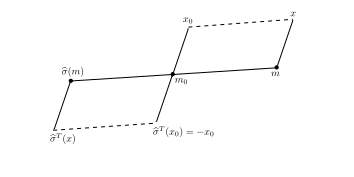
\includegraphics{chap3-fig1}
\end{figure}
\end{itemize}
\end{proof}

\begin{remark*}
The transformation $\widehat{\sigma}$ defined above is called {\em the
  symmetry around} $m_{0}$. By \eqref{chap3:3.3.10} it follows that it is an
involution having $m_{0}$ as isolated fixed point. Since $G$ acts
transitively on $M$, given any point $m$ of $M$, there exists an $a$
of $G$ such that
$$
\tau(a)(m_{0})=m.
$$\pageoriginale
Then we see that the transformation
\begin{equation*}
\tau(a)\circ\widehat{\sigma}\circ\tau(a)^{-1}\tag{3.3.16}\label{chap3:3.3.16}
\end{equation*}
is an involution having $m$ as isolated fixed point. We call this
involution the {\em symmetry around} $m$ and denote it by
\begin{equation*}
\widehat{\sigma}_{m}.\tag{3.3.17}\label{chap3:3.3.17}
\end{equation*}
\end{remark*}

Concerning these symmetries we have the following:

\setcounter{subsection}{17}

\subsection{}\label{chap3:3.3.18}

\begin{prop*}
If $m$, $m'\in M$ are sufficiently near then $\exists\, n\in M$ such that
$$
\widehat{\sigma}_{n}(m)=m'.
$$
\end{prop*}

\begin{proof}
Since $G$ acts transitively on $M$ we can suppose that $m=m_{0}$. Now
since the map
$$
p^{T}\circ
(\exp|\underbar{M})^{T}:\underbar{M}\xrightarrow{(\exp|\underbar{M})^{T}} T_{e}(G)\xrightarrow{p^{T}}T_{m_{0}}(N),
$$
is an isomorphism, the inverse function theorem shows, since $m'$ is
close enough to $m_{0}$; that there exists an $X\in\underbar{M}$ such
that
$$
m'=\exp(X).
$$
Now $p(\exp(\dfrac{X}{2}))$ can be taken for $n$.
\end{proof}

\setcounter{subsection}{18}
\subsection{}\label{chap3:3.3.19}
The homogeneous Riemannian manifold $(M,\gamma)$ is called the {\em
  symmetric space} associated to the symmetric pair $(G,H)$.

\setcounter{subsection}{19}

\subsection{}\label{chap3:3.3.20}


\begin{remark*}
1.~Let
$$
f:t\to \exp(tX).
$$
Then \pageoriginale from the above proof it is clear that
$$
\widehat{\sigma}_{f(t_{0})}(f(t))=f(2t_{0}-t).
$$
\end{remark*}

\subsection{}\label{chap3:3.3.21}

\begin{remark*}
2.~In fact, the condition that $m$ and $m'$ be sufficiently near is
superfluous: (see \ref{chap4:4.4.3}).
\end{remark*}

\section{The S.C.-manifolds}\label{chap3:sec4}

\quad 
By $K$ we denote one of the following fields: $\mathbb{R}$ (the real
numbers), $\mathbb{C}$ (the complex numbers), $\mathbb{H}$ (the
quaternions); the conjugation in $K$ is $z\to \overline{z}$ and we set
$k=\dim_{\mathbb{R}} K(k=1,2,4)$. We, consider $K^{n}$ (for an integer
$n$) as a 
left vector space over $K$, denote by $e_{1},\ldots,e_{n}$ its
canonical basis and use freely the two identifications:
\begin{gather*}
K^{n+1}=K^{n}\times
K:(z_{1},\ldots,z_{n},z_{n+1})=(z=(z,\ldots,z_{n}),z_{n+1})=(z,z_{n+1}).\\
K^{n}\subset
K^{n+1}:(z_{1},\ldots,z_{n})=(z_{1},\ldots,z_{n},0).\tag{3.4.1}\label{chap3:3.4.1} 
\end{gather*}
On $K^{n}$ we consider the canonical hermitian structure $<,>$:
$$
<(z_{1},\ldots,z_{n}),(w_{1},\ldots,w_{n})>=\sum_{i}z_{i}\overline{w}_{i}.
$$
By $\mathbb{U}(K^{n})$ we denote the set of all $K$-endomorphisms of
$K^{n}$ which leave $<,>$ invariant; for $K=\mathbb{R}$, $\mathbb{C}$
we denote by $\mathbb{S}\mathbb{U}(K^{n})$ the subgroup of
$\mathbb{U}(K^{n})$ of elements of determinant equal to one. We also
set:
\begin{align*}
S0(n)&=\mathbb{S}\mathbb{U}(\mathbb{R}^{n}),0(n)=\mathbb{U}(\mathbb{R}^{n}).\tag{3.4.2}\label{chap3:3.4.2}\\
SU(n) &=
\mathbb{S}\mathbb{U}(\mathbb{C}^{n}),U(n)=\mathbb{U}(\mathbb{C}^{n}),n\geq
1\tag{3.4.2}\\
Sp(n) &= (\mathbb{S}\mathbb{U}(\mathbb{H}^{n})=)\mathbb{U}(\mathbb{H}^{n}).
\end{align*}\pageoriginale
All these are compact Lie groups, and, with the exception of $0(n)$,
all are connected. The component of the identity of $0(n)$ is $S0(n)$.

\setcounter{subsection}{2}

\subsection{}\label{chap3:3.4.3}

\begin{prop*}
$\mathbb{S}\mathbb{U}(K^{n})$ acts transitively on the $K$-directions
  and also on the $\mathbb{R}$-directions of $K^{n}$; also $S0(n)$
  acts transitively on the planes of $\mathbb{R}^{n}$; if
  $K=\mathbb{C}$, then $n>1$.
\end{prop*}

In particular $\mathbb{S}\mathbb{U}(K^{n})$ acts transitively on the
sphere
\begin{equation*}
\mathbb{S}(K^{n})=\{x\in
K^{n}|<x,x>=1\};\mathbb{S}^{n}=\mathbb{S}(\mathbb{R}^{n+1}).\tag{3.4.5}\label{chap3:3.4.5}   
\end{equation*} 
On $K^{n+1}-0$ the equivalence relation $R:z {\sim} z'$ if and only if
$\exists\, \lambda\in K$ with $z=\lambda z'$ yields the {\em
  projective space}
\begin{equation*}
P^{n}(K)=(K^{n+1}-\{0\})/R,\quad 
\vcenter{\xymatrix{
K^{n+1}-\{0\}ar[d]_{p}\\
P^{n}(K)
}}\tag{3.4.6}\label{chap3:3.4.6}
\end{equation*}
on which $\mathbb{S}\mathbb{U}(K^{n+1})$ acts transitively. So
$P^{n}(K)$ is a homogeneous space; and is a connected compact
manifold, of dimension k.n. We write $P^{n}(K)=M=G/H$ where
$G=\mathbb{S}\mathbb{U}(K^{n+1})$ and $H$ is the subgroup of $G$
leaving the point $m_{0}=p(e_{n+1})$ fixed. We set
\begin{equation*}
H=\mathbb{S}(\mathbb{U}(K^{n})\times\mathbb{U}(K))=\mathbb{S}\mathbb{U}(K^{n+1})\cap
(\mathbb{U}(K^{n})\times\mathbb{U}(K))\tag{3.4.7}\label{chap3:3.4.7} 
\end{equation*}
where $\mathbb{U}(K^{n})\times\mathbb{U}(K)$ is embedded in
$\mathbb{U}(K^{n+1})$ by \eqref{chap3:3.4.1}. For elements of $H$ we use the
notation $(f,\widehat{\lambda})$ where $f\in \mathbb{U}(K^{n})$ and
$\widehat{\lambda}\in\mathbb{U}(K)$ stands for the map
$\mu\to\mu\lambda$ of $K$ into itself which is \pageoriginale
associated to the element $\lambda\in K$ (with $<\lambda,\lambda>=1$),
i.e.
\begin{equation*}
(f,\widehat{\lambda})(z,z_{n+1})=(f(z),z_{n+1}\lambda).\tag{3.4.8}\label{chap3:3.4.8} 
\end{equation*}
From \eqref{chap3:3.4.7} and \eqref{chap3:3.4.7} we get the fibrations:
\begin{equation*}
\vcenter{\xymatrix{
\mathbb{S}^{n}\ar[d]^{\mathbb{Z}_{2}}\ar@{}[r] &
\mathbb{S}^{2n+1}\ar[d]^{\mathbb{S}^{1}}\ar@{}[r] &
\mathbb{S}^{4n+3}\ar[d]^{\mathbb{S}^{3}}\\
P^{n}(\mathbb{R}) & P^{n}(\mathbb{C}) & P^{n}(\mathbb{H})
}}
\tag{3.4.10}\label{chap3:3.4.10}
\end{equation*}
We show now that $(G,H)$ is canonically a symmetric pair; define an
endomorphism $s$ of $K^{n+1}$ and an automorphism $\sigma$ of $G$ by:
\begin{equation*}
\begin{split}
& s(e_{i})=e_{i}\text{ \ for \ } i=1,\ldots,n\text{ \ and \ } s(e_{n+1})=-e_{n+1}\\
& \sigma:g\to \sigma(g)=s\circ g\circ s.
\end{split}\tag{3.4.11}\label{chap3:3.4.11}
\end{equation*}
As is easily verified, the subgroup of elements fixed under $\sigma$
is nothing but $H=\mathbb{S}(\mathbb{U}(K^{n})\times\mathbb{U}(K))$.

We study now the complement $\underbar{M}$ in
$G=\underbar{H}+\underbar{M}$ as defined in (\ref{chap3:sec3}), by
introducing the map $r:K^{n}\to \underbar{G}$ defined by:
\begin{align*}
r(z)(e_{n+1})=z, r(z)(z)=-e_{n+1},r(z)(u) &=
0\tag{3.4.12}\label{chap3:3.4.12}\\
 \forall u|<u,z> &= 0
\end{align*}
when $<z,z>=1$ and extension by linearity. Hence the one-parameter
subgroup of $G$ associated to $r(z):t\to \exp(t\cdot r(z))$ is nothing
but:
\begin{equation*}
\exp(t\cdot r(z)):
\begin{cases}
e_{n+1}\to (\cos t)e_{n+1}+(\sin t)z\\
z\to -(\sin t)e_{n+1}+(\cos t)z\\
u\to u \, \forall u\text{ \ with \ } <u,z>=0.
\end{cases}\tag{3.4.13}\label{chap3:3.4.13}
\end{equation*}
Remark that $\dim(K^{n})=k.n=\dim G/H=\dim\underbar{M}$ and that
$r(K^{n})\subset \underbar{M}$ for a direct computation yields:
$$
(\exp(t.r(z))=\exp(-t.r(z)).
$$\pageoriginale
Hence:
\begin{equation*}
r(K^{n})=\underbar{M},p^{T}\circ r:K^{n}\to
T_{m_{0}}(M)\tag{3.4.14}\label{chap3:3.4.14} 
\end{equation*}
is an isomorphism. To find the action of $\Ad H$ on $\underbar{M}$ we
use \eqref{chap3:3.3.9} and \eqref{chap3:3.4.14}. To $z\in K^{n}$ we associate the
curve $l:t\to p(e_{n+1}+tz)$ in $P^{n}(K)$. For the image
$\tau(h)\circ l$ under $h=(f,\widehat{\lambda})\in H$, by
\eqref{chap3:3.4.8} and definition of $P^{n}(K)$ we have: 
\begin{align*}
t\to\tau (h)(p(e_{n+1}+tz)) &= p(h(e_{n+1}+tz))=p(\lambda\cdot
e_{n+1}+t\cdot f(z))=\\
&= p(e_{n+1}+t\cdot\lambda^{-1}\cdot f(z))
\end{align*}
hence by (\ref{chap0:0.5.7}) and \eqref{chap3:3.3.9}:
\begin{align*}
(\tau(h)\circ l)'(0) &= (p^{T}\circ r)(\lambda^{-1}\cdot
  f(z))=(\tau(h))^{T}(l'(0))=\\ 
&= ((\tau(h))^{T}\circ p^{T}\circ r)(z)=(p^{T}\circ \Ad(h))(r(z))
\end{align*}
which yields:
\begin{equation*}
\Ad((f,\widehat{\lambda}))=r\circ (\lambda^{-1}f)\circ
r^{-1}.\tag{3.4.15}\label{chap3:3.4.15} 
\end{equation*}

\setcounter{subsection}{15}
\subsection{}\label{chap3:3.4.16}


\begin{remarks*}
In the case $K=\mathbb{R}$, $\mathbb{C}$ the {\em homomorphism}
$H=\mathbb{S}(\mathbb{U}(K^{n})\times\mathbb{U}(K)))\to
\mathbb{U}(K^{n})$ defined by $(f,\widehat{\lambda})\to
\lambda^{-1}\cdot f$ in onto because the condition
$(f,\widehat{\lambda})\in \mathbb{S}\mathbb{U}(K^{n+1})$ is equivalent
to the condition $\lambda\cdot \det f=1$, so that $\lambda^{-1}\cdot
f=(\det f)\cdot f$ (and this is injective when $n>1$.). This explains
why one sometimes writes: $P^{n}(\mathbb{R})=S0(n+1)/0(n)$;
$P^{n}(\mathbb{C})=SU(n+1)/U(n)$. One also writes:
$$
P^{n}(\mathbb{H})=\Sp(n+1)/\Sp(n)\times \Sp(1)
$$
which is correct because
$\mathbb{S}\mathbb{U}(\mathbb{H}^{n})=\mathbb{U}(\mathbb{H}^{n})$. For
the sphere $S0(n+1)/S0(n)$ the computation as above (except that there
is no projection $p$) shows that $\Ad H$ is isomorphic to the action
of $S0(n)$ in \pageoriginale $\mathbb{R}^{n}$ (under
\eqref{chap3:3.4.1}). From these remarks and from (\ref{chap3:3.4.3}) we get:
\end{remarks*}

\subsection{}\label{chap3:3.4.17}

\begin{prop*}
For $P^{n}(K)=G/H$ the action of $\Ad H$ is transitive on the
directions of $\underbar{M}$; for $P^{n}(\mathbb{R})$ or
$\mathbb{S}^{n}$ the action of $\Ad H$ is transitive on the planes of
$\underbar{M}$.
\end{prop*}

In particular $\Ad H$ acts irreducibly on $\underbar{M}$ so by
(\ref{chap3:3.3.12}) there exists (upto a positive constant) a canonical
r.s.\@ on $G/H$; in fact there exists a {\em canonical} r.s.\@ on
$G/H$, for we see from \eqref{chap3:3.4.14} and \eqref{chap3:3.4.15} that the
canonical euclidean structure on $K^{n}$ (deduced from its canonical
hermitian form) gives a euclidean structure on $\underbar{M}$
invariant by $\Ad H$. So we require by definition, that: 

\subsection{}\label{chap3:3.4.18} 
$r:K^{n}\to \underbar{M}$ be a euclidean isomorphism. {\em We
  write} ($P^{n}(K)$, can) {\em for this symmetric space} and leave
the reader to check in the case of $\mathbb{S}^{d}=S0(d+1)/S0(d)$ that
this procedure yields nothing but ($\mathbb{S}^{d}$, can) as defined
in \ref{chap3:3.2.1}.

\setcounter{subsection}{18}

\subsection{}\label{chap3:rems3.4.19}

\begin{remarks*}
we leave to the reader the proofs of the following facts:
\begin{enumerate}
\renewcommand{\theenumi}{\Alph{enumi}}
\renewcommand{\labelenumi}{\theenumi)}
\item the imbedding $K^{n}\to K^{n+1}$ yields an imbedding of
  $p^{n-1}(K)$ as a sub manifold of $P^{n}(K)$. Prove the canonical
  r.s.\@ on the $P^{n}(K)$'s are {\em hereditary} in the sense that
  the induced r.s.\@ on $P^{n-1}(K)$ by the canonical r.s.\@ of
  $P^{n}(K)$ is its canonical r.s.;

\item the first fibration in \eqref{chap3:3.4.10} is a riemannian
  covering. The two last ones are excellent in the sense that for 
\[
\xymatrix@C=.05cm@R=.5cm{
 & E\ar[dd] &\\
F & & P\\
 & B &
}
\]\pageoriginale
first the r.s.\@ induced on the fibres is the canonical one; second:
if one writes at any $m\in E$ the orthogonal decomposition
$$
T_{m}(E)=T_{m}(p^{-1}(p(m)))+N
$$
then $p^{T}N:N\to T_{p(m)}(B)$ is a euclidean isomorphism.
\end{enumerate}
\end{remarks*}

To those symmetric spaces we add the symmetric space
$P^{2}(\Gamma)=F_{4}/\Spin(9)$ {\em the Cayley projective plane} (see:
\cite{37}). We consider on it the canonical r.s.\@ ($P^{2}(\Gamma)$,
can) such that all its geodesics are closed and of length $\pi$ (see
\cite{14}, p.356). 

\setcounter{subsection}{19}

\subsection{}\label{chap3:3.4.20}

\begin{defi*}
Any of the ($P^{n}(K)$, can), ($\mathbb{S}^{d}$, can),
($P^{2}(\Gamma)$, can) is called as {\em S.C.-manifold}.
\end{defi*}

We will use also a non compact symmetric space defined as follows. Let
$S0_{0}(d,1)$ be the identity component of the linear group of
$\mathbb{R}^{d+1}$ which leaves invariant the quadratic form:
$$
(x_{1},\ldots,x_{d},x_{d+1})\to x^{2}_{1}+\cdots+x^{2}_{d}-x^{2}_{d+1}
$$
For the same $s$ and $\sigma$ as in \eqref{chap3:3.4.2} we get the symmetric
pair $(G,H)=(S0_{0}(d,1),S0(d))$. Again $S0(d)$ acts by $\Ad$ on
$\underbar{M}$ as $S0(d)$ on $\mathbb{R}^{d}$; in particular:

\setcounter{subsection}{20}
\subsection{}\label{chap3:3.4.21}
$\Ad H$ acts transitively on the planes of $\underbar{M}$.

In particular by \ref{chap3:3.3.12} we get (upto a positive constant) a
canonical r.s.\@ on $M=G/H$. In fact $M$ is homeomorphic to
$\mathbb{R}^{d}$; for,
\begin{equation*}
A=\{z=(x_{1},\ldots,x_{d}x_{d+1})\in\mathbb{R}^{d+1}|x_{d+1}\geq
0,<z,z>=1\}\text{ \ and}
\end{equation*}
define \pageoriginale the injection 
$$i:A\to P^{d}(\mathbb{R}) \mbox{ by }
i(x_{1},\ldots,x_{d},x_{d+1})=p(x_{1},\ldots,x_{d},1).$$

\begin{claim*}
$S0_{0}(d,1)$ acts transitively on $i(A)$; in fact, for any $z$ with
  $<z,z>=1$, we have in $S0_{0}(d,1)$ the one parameter subgroup 
$$
t\to g(t)
\begin{cases}
e_{n+1}\to (ch\, t)\cdot e_{n+1}+(sh\, t)\cdot z\\
z\to (sh\, t)\cdot e_{n+1}+(ch\, t)\cdot z\\
u\to u\forall u\text{ \ with } <u,z>=0,
\end{cases}
$$
so that
\begin{align*}
g(t))(p(e_{n+1})) &= p(g(t)(e_{n+1})=p(ch\, t)\cdot e_{n+1}+(sh\,
t)\cdot z)=\\
&= p(e_{n+1}+(th\, t)\cdot z).
\end{align*}
Having an r.s.\@ on $i(A)$, we use a diffeomorphism between $A$ and
$\mathbb{R}^{d}$ to get a canonical r.s.\@ on $\mathbb{R}^{d}$ which
we denote by $(\mathbb{R}^{d},\hyp)$.
\end{claim*}

\setcounter{subsection}{21}
\subsection{}\label{chap3:3.4.22}
$(\mathbb{R}^{d},\hyp)$ is called the {\em hyperbolic space of
  dimension $d$.}

\section{Volumes}\label{chap3:sec5}

\quad 
Let $(M,g)$ be an r.m. Then for every $m\in M$, $T_{m}(M)$ has a
euclidean structure by $g$ i.e.\@ the one given by the symmetric
positive definite bilinear form $g_{m}$. Hence it has a canonical
volume (see \ref{chap0:0.3.6}) $t_{m}$, and further if $(M,g)$ is oriented
then $T_{m}(M)$ admits a canonical volume form $S_{m}$ induced by the
oriented form $\sigma'$, i.e. the orientation given by $\sigma'_{m}$.

\subsection{}\label{chap3:3.5.1}

\begin{prop*}
With \pageoriginale the above notation the map
$$
\theta:m\to t_{m}
$$
is a volume element on $M$ (called canonical volume element on
  $M$) and if $M$ is oriented the map  
$$
\sigma:m\to S_{m}
$$
is a volume form (called the canonical volume form).
\end{prop*}

\begin{proof}
Let us consider the second case first. We know that for
{\small $X_{1},\ldots,X_{d}$} belonging to $\mathscr{C}(M)$,
$\sigma(X_{1},\ldots,X_{d})$ is $F(M)$-multilinear. Hence to show that
$\sigma$ is a volume form we need only show that
$\sigma(X_{1},\ldots,X_{d})$ is differentiable. To see this, since
differentiability is a local property, let $(U,r)$ be a chart of $M$,
and let $Y_{1},\ldots,Y_{d}$ be a basis of $\mathscr{C}(U)$,
orthonormal relative to the restriction of $g$ to $U$. We can suppose
that $Y_{i}$ in that order are positive relative to $\sigma'$. Then we
have
$$
\sigma(Y_{1},\ldots,Y_{d})(m)=1,\forall m\in U,
$$
and hence, since $\sigma$ is $F(M)$-multilinear, it is differentiable
on $U$.
\end{proof}

Now let us take up the first part. We know that $t_{m}$ is a volume
element on $T_{m}(M)$. So to show that $\theta$ is a volume element,
it is enough to show that $\theta$ is, locally the modulus of a volume
form. To see this let us take an orientation $\sigma'_{1}$ on $U$ and
then, clearly,
$$
\theta=|\sigma_{1}|,
$$
where $\sigma_{1}$ is related to $\sigma'_{1}$ as $\sigma$ is to
$\sigma'$.

\setcounter{subsection}{1}
\subsection{}\label{chap3:3.5.2}\pageoriginale

Let us note that if \; $\{X_{1},\ldots,X_{d}\}$ is any local basis of
$\mathscr{C}(M)$ the formula (\ref{chap0:0.3.6}) gives
$$
\theta(X_{1},\ldots,X_{d})=(\det(g(X_{i},X_{j})))^{\frac{1}{2}}.
$$
If $(M,g)$ is a compact manifold then we know that
$$
\int\limits_{M}\theta
$$
exists. We call this number the {\em volume of $(M,g)$ and denote it
  by Vol $(M,g)$.} Generally, if no confusion is possible, we omit the
reference to $g$ and say the volume of $M$ and write $\Vol(M)$. If the
dimension of the manifold is one, volume is called length and if it is
two volume is called area. They are denoted by $lg(M)$ and $ar(M)$
respectively.

Let us note that in the oriented case, with the notation of
(\ref{chap3:3.5.1}),
$$
\int\limits_{M}\theta =\int\limits_{M}\sigma
$$
If $N$ is a compact sub manifold of $M$ then there is an induced r.s.\@
on $N$ (see (\ref{chap3:3.2.1})) A). Whenever we talk of volume of $N$
without any reference to the r.s.\@ on $N$ this induced structure is
the one that is considered. {\em And further, we set:
  $\Vol(N,g|N)=\Vol(N)$.}

\subsection{}\label{chap3:3.5.3}

In particular, suppose the dimension of $N$ is equal to one; then if
$N$ admits the parametric representation $N=f(I)$ where $I=[0,1]$ and
$f$ is a curve $f:I\to M$, we have:
$$
lg(f(I))=\int\limits_{f(I)}\lambda=\int\limits_{I}f^{\ast}\lambda =
\int\limits^{1}_{0}(f^{\ast}\lambda)(P)  
$$
where \pageoriginale $\lambda$ is the length form of $(N,g|N)$. But 
$(f^{\ast}\lambda)(P)=\lambda(f^{T}\circ P)= \lambda(f')=||f'||$ so
that
$$
lg(N)=\int\limits^{1}_{0}||f'||\dt=lg(f(I)).
$$
This leads to the following definition for paths (and a fortiori for
curves):

\begin{defi*}
Let $C=\{f_{i}\in D(I_{i},M), [a_{i},b_{i}]\subset I_{i}\}$ be a path
in an r.m.\@ $(M,g)$. Then {\em the length of $C$, denoted by $lg(C)$,}
is by definition:
$$
lg(C) = \sum_{i}\int\limits^{b_{i}}_{a_{i}} ||
f'_{i}||\dt=\sum_{i}lg(f_{i}[a_{i},b_{i}]).  
$$
\end{defi*}

Now let us examine the volume element more closely.

\subsection{}\label{chap3:3.5.4}

Let $(M,g)$ be an r.m.\@ and let $\varphi$ be a differentiable
function on $M$ which is everywhere positive. Then $\varphi g$ defined
by the equation
$$
\varphi\cdot g(X,Y)=\varphi(p_{M}(X))\cdot g(X,Y),X,Y\in\mathscr{C}(M)
$$
defines an r.s.\@ on $M$. If we denote the volume element of
$(M,\varphi,g)$ by $\theta_{\varphi}$ and that of $M$ by $\theta$
then, from (\ref{chap3:3.5.2}) it follows that they are related by the
equation
$$
\theta_{\varphi}=\varphi^{d/2}\cdot\theta
$$

\subsection{}\label{chap3:3.5.5}
B.~Let $(M,g)$ and $(N,h)$ be two compact r.m.'s which are
isometric. They by the definitions of isometry, volume and by
(\ref{chap0:0.3.9}) we have $\Vol(M,g)=\Vol(N,h)$.

\subsection{}\label{chap3:3.5.6}\pageoriginale

C.~Let $(M,g)$ and $(N,h)$ be two r.m.'s and let
$$
p:(M,g)\to (N,h)
$$
be a riemannian covering. Further let us suppose that $N$ is compact
and the covering has a finite number, $k$, of sheets. Then $\Vol(M,g)$
exists and further
$$
\Vol(M,g)=k,\Vol(N,h).
$$
To see this let us take an open covering $\{(U_{i},r_{i})\}$ by
coordinate neighbourhoods of $N$, $U_{i}$ taken so small as to make
$p^{-1}(U_{i})$ the union of $k$ disjoint components
$U_{i_{1}},\ldots,U_{i_{k}}$ (this is possible because $p$ is a
$k$-sheeted covering map.) Then $\{U_{i_{j}},r_{i_{j}}=r_{i}\circ
p|U_{ij}\}$ is a complete atlas for $(M,g)$. Now let us take a
partition of unity $\{\varphi_{i}\}$ on $N$ subordinate to the
covering $U_{i}$. Then $\psi_{i_{j}}$ defined by
$$
\psi_{i_{j}}=
\begin{cases}
\varphi_{i}\circ p\text{ \  on \ } U_{i_{j}}\\
0\text{ \ outside \ } U_{i_{j}}
\end{cases}
$$
is a partition of unity on $M$ subordinate to the covering
$\{U_{i_{j}}\}$. Now since $p$ is a riemannian covering map, denoting
the volume element of $(M,g)$ and $(N,h)$ by $\theta_{M}$ and
$\theta_{N}$ respectively, we have
\begin{align*}
\int\limits_{U_{i_{j}}}\psi_{i_{j}}\theta_{M} &=
\int\limits_{U_{i_{j}}}(\varphi_{i}\circ
p)(p^{\ast}\theta_{N})=\int\limits_{U_{i_{j}}}p^{\ast}(\varphi_{i}\theta)\\
&\qquad =\int\limits_{U_{i}}\varphi_{i}\theta\text{ by } (3.5.5).
\end{align*}
Hence\pageoriginale
\begin{align*}
\Vol(M,g) &=
\sum_{j}(\sum_{i}\int\limits_{U_{i_{j}}}\psi_{i_{j}}\theta_{M})=\sum_{j}(\int\limits_{N}\theta)\\
&= k.\Vol(N,h).
\end{align*}
Now let us note a particular case. If we take the real projective
space ($P^{d}(\mathbb{R})$, can) for $(N,h)$ and ($\mathbb{S}^{d}$,
can) for $(M,g)$ and the natural map of $\mathbb{S}^{d}$ onto
$P^{d}(\mathbb{R})$ for $p$ then we have $k=2$. Hence
$$
\Vol(P^{d}(\mathbb{R}),\can)=\frac{1}{2}\Vol(\mathbb{S}^{d},\can).
$$

\subsection{}\label{chap3:3.5.7}
D.~Let us consider the case of a flat torus $\mathbb{R}^{d}/G$ (see
(\ref{chap3:3.2.2}) D.2). Let $(\tau_{1},\ldots,\tau_{d})$ be a set of
generators for $G$. Then $\tau_{1}(0),\ldots,\tau_{d}(0)$ is a basis
of $\mathbb{R}^{d}$. Let $(v_{1},\ldots,v_{d})$ be the corresponding
coordinate system. Now let
$$
W=\{x\in\mathbb{R}^{d}|0<v^{i}(x)<1,\text{ \ for \ } i=1,\ldots,d\}.
$$
Then $W$ is open in $\mathbb{R}^{d}$, $\overline{W}$ is compact and
the restriction of 
$$
p:\mathbb{R}^{d}\to \mathbb{R}^{d}/G
$$
to $W$ is a diffeomorphism of $W$ with $p(W)$. Also
$p(\overline{W})=\mathbb{R}^{d}/G$ and $\overline{W}-W$ is of measure
zero. Hence
\begin{align*}
&\Vol(R^{d}/G,\epsilon/G)=\Vol(p(W),\epsilon/G)=\\
&=\Vol(W,\epsilon)=|\det(\tau_{1}(0),\ldots,\tau_{d}(0))|\text{ by }\;
    (\tag{chap0:0.3.2}).
\end{align*}

\section{The canonical forms $\alpha$ and $d\alpha$}\label{chap3:sec6}

Let $(M,g)$ be an r.m. Then there is a map
$$
g^{\sharp}:\mathscr{C}(M)\to \mathscr{C}^{\ast}(M)
$$
given \pageoriginale by the equation
$$
g^{\sharp}(X)(Y)=g(X,Y),\forall Y\in \mathscr{C}(M).
$$
Clearly it is an $F(M)$-linear map and since $g$ is non-degenerate it
follows that $g^{\sharp}$ is an isomorphism of $F(M)$-modules. Let us
note that
$$
g^{\sharp}(X)=i(X)g.
$$

\subsection{}\label{chap3:3.6.1}
We set $g^{\flat}=(g^{\sharp})^{-1}$. Now evaluating $g^{\sharp}$ at
each point of $T(M)$ we get a vector bundle isomorphism of $T(M)$ with
$T^{\ast}(M)$. We denote this map also by the symbol $g^{\sharp}$ and
it will be clear from the context which we mean by $g^{\sharp}$.
\begin{equation*}
\vcenter{\xymatrix@R=1.7cm@C=1.2cm{
T(M)\ar@{-}@<-.3em>[rr]_{g^{\flat}}\ar@{-}@<.3em>[rr]^{g^{\sharp}}\ar[dr]_{p} & & 
T^{\ast}(M)\ar[dl]^{p^{\ast}}\\
 & M & 
}}\tag{3.6.2}\label{chap3:3.6.2}
\end{equation*}

\setcounter{subsection}{2}

\subsection{}\label{chap3:rem3.6.3}

\begin{remark*}
Let us note that $g^{\sharp}$ and $g^{\flat}$ give rise, in a natural,
way, to isomorphisms of 
$$
\mathscr{L}^{r\pm i}_{s\mp i}\quad\text{with}\quad \mathscr{L}^{r}_{s}
$$
between tensor spaces over $(M,g)$ (these isomorphisms describe the
operation usually called ``raising'' or ``lowering'' subscripts).
\end{remark*}

Now \pageoriginale we utilise the maps $g^{\flat}$ and $g^{\sharp}$ to
associate an 
element of $\mathscr{C}(M)$ with every $\varphi$ and to pull $\mu$
from $T^{\ast}(M)$ to $T(M)$ where $\mu$ is defined in (\ref{chap0:0.4.24}).

\subsection{}\label{chap3:3.6.4}


\begin{defi*}
For every $\varphi\in F(M)$ we set
$$
\grad \varphi=g^{\flat}(d\varphi).
$$
If $U$ is an open subset of $(\mathbb{R}^{d},\epsilon)$ and
$\varphi\in F(U)$ then we have
$$
\grad \varphi=\sum_{i}\frac{\partial\varphi}{\partial
  u^{i}}\frac{\partial}{\partial u^{i}}.
$$
\end{defi*}


\subsection{}\label{chap3:3.6.5}

\begin{defi*}
$\alpha=(g^{\sharp})^{\ast}(\mu)$.

If we have to consider the $\alpha$'s associated to several manifolds
$(M,g)$, $(N,h),\ldots$ at the same time, we write $M_{\alpha}$,
$N_{\alpha}$ for the corresponding $\alpha$'s.
\end{defi*}

\setcounter{subsection}{5}
\subsection{}\label{chap3:3.6.6}
For every $z$ in $T(T(M))$ we have
$$
\alpha(z)=g(p'(z),p^{T}(z)).
$$

\begin{proof}
For
\begin{align*}
\alpha(z) &= (g^{\sharp})^{\ast}(\mu(z))=\mu(g^{\sharp T}(z))=\\
          &= (p''(g^{\sharp T}(z))=(p^{\ast T}(g^{\sharp T}(z)).
\end{align*}
\[
\xymatrix@C=1.5cm@R=1.2cm{
T(T(M))\ar[rr]_{(g^{\sharp})^{T}}\ar[d]_{p'} & &
T(T^{\ast}(M))\ar[d]^{p''}\\
T(M)\ar[rr]^{g^{\sharp}}\ar[dr]_{p} & &
T^{\ast}(M)\ar[dl]^{p^{\ast}}\\
 & M & 
}
\]
But \pageoriginale $p^{\ast T}\circ g^{\sharp T}=(p^{\ast}\circ
g^{\sharp})^{T}=p^{T}_{M}$ and $p''\circ g^{\sharp T}=g^{\sharp}\circ
p_{M}$. Hence
$$
(z)=(g^{\sharp}\circ p'_{M}(z))(p^{T}(z))=g(p'(z),p^{T}(z)).
$$
\end{proof}

\subsection{}\label{chap3:3.6.7}
If $f:(M,g)\to (N,h)$ is an isometry, then
$$
M_{\alpha=(f^{T})^{\ast}({}^{N}(\alpha))}\quad\text{and}\quad
  d({}^{M}\alpha)=(f^{T})^{\ast}(d({}^N\alpha)). 
$$

\begin{proof}
In view of the formula (\ref{chap0:0.2.9}) IV. We need only prove the first
equality. We have, by (\ref{chap3:3.6.6}),
\begin{gather*}
M_{\alpha(z)=g(p'_{M}(z), p^{T}_{M}(z))}\quad\text{and}\\
(f^{T})^{\ast}({}^{N}\alpha)(z)={}^{N}\alpha(f^{T}(z))=h(p'_{N}(f^{T})^{T}(z)),
p^{T}_{M}(f^{T})^{T}(z) 
\end{gather*}
\[
\xymatrix@R=1.7cm@C=2.2cm{
T(T(M))\ar[r]^{(f^{T})^{T}}
\ar@<.25em>[d]^{p'_{M}}\ar@<-.25em>[d]_{p^{T}_{M}} &
T(T(N))\ar@<.3em>[d]^{p^{T}_{N}}\ar@<-.3em>[d]_{p'_{N}}\\
T(M)\ar[r]^{f^{T}}\ar[d]^{p_{M}} & T(N)\ar[d]^{p_{N}}\\
M\ar[r]^{f} & N
}
\]
But we have
$$
p'_{N}\circ (f^{T})^{T}=f^{T}\circ p'_{M}\quad\text{and}\quad
p^{T}_{N}\circ (f^{T})^{T}=f^{T}\circ p^{T}_{M}.
$$
Hence\pageoriginale
\begin{align*}
f^{T^{\ast}}({}^{N}\alpha) &=
h(f^{T}(p'_{M}(z)),f^{T}(p^{T}_{M}(z))=\\
&= (f^{\ast}h)(p'_{M}(z),p^{T}_{M}(z))=\\
&= g(p'_{M}(z),p^{T}_{M}(z))\text{ \ since $f$ is an isometry.}
\end{align*}
Hence the result.
\end{proof}

Since $g^{\sharp}$ is an isomorphism so is $(g^{\sharp})^{\ast}$. Now
by lemma (\ref{chap0:0.4.27}) we get the following result.

\subsection{}\label{chap3:3.6.8}

\begin{prop*}
$d\alpha$ is non-degenerate everywhere on $T(M)$.
\end{prop*}

\setcounter{subsection}{8}
\subsection{}\label{chap3:3.6.9}
In particular it follows that
${\displaystyle{\mathop{\wedge}^{\alpha}}}d\alpha$ is a volume form for
  $T(M)$ (see also (\ref{chap5:5.2.5})).

\subsection{}\label{chap3:3.6.10}


\begin{lemma*}
For every $x\in T(M)$, $z\in V_{x}$ and $z'\in T_{x}(T(M))$ we have
$$
(d\alpha)(z,z')=g(\xi(z),p^{T}(z')).
$$
\end{lemma*}

\begin{proof}
Let us choose $Z$ and $Z'$ in $\mathscr{C}(T(M))$ such that
\begin{itemize}
\item[i)] $p^{T}(Z)=0$ and $Z(x)=z$ (for example let us take any
  $Y\in\mathscr{C}(M)$ such that $Y(p(x))=\xi(z)$ and set
  $Z(x)=\xi^{-1}_{U}(Y(p(U))$ for every $U$ in $T(M)$); and

\item[ii)] there exists an $X$ in $\mathscr{C}(M)$ for which
  $p^{T}(Z')=X$; (for example let us take any $Y$ in $\mathscr{C}(M)$
  such that $Y(p(x)=p^{T}(z')$ and set $Z'=Y^{T}$ (see
  (\ref{chap0:0.4.19})).
\end{itemize}
Then
\begin{align*}
d\alpha (z,z') &= (d\alpha)(Z,Z')_{x}\\
               &= Z(\alpha(Z'))_{x}-Z'(\alpha(Z))_{x}-\alpha([Z,Z'])_{x}.
\end{align*}
But \pageoriginale by (\ref{chap3:3.6.6}) we have
$$
(Z)=g(p'\circ Z',p^{T}\circ Z)=g(p'\circ Z,0)=0;
$$
\begin{align*}
\alpha([Z,Z]) &= g(p'\circ[Z,Z'],p^{T}\circ [Z,Z'])\\
              &= g(p'\circ[Z,Z'],[p^{T}(Z),p^{T}(Z')])\\
              &= g(p\circ[Z,Z'],0)=0,
\end{align*}
and
\begin{gather*}
\alpha(Z')=g(p'\circ Z',p^{T}\circ Z')=g(\id)T(M),p^{T}\circ Z'),\\
\text{i.e. \ } \alpha(Z')_{y}=g(y,(p^{T}\circ Z')(p(y)).\text{
  \ Hence}\\
d\alpha(z,z')=Z(\alpha(Z'))_{x}=z(\alpha(Z')).
\end{gather*}
Now let us consider the map of $T(M)$ into $\mathbb{R}$ defined by
$$
T(M)\to y\to \alpha(Z')_{y}=g(y,X(p(y)).
$$
Clearly it is a linear function on $T(M)$. Hence, by (\ref{chap0:0.4.16}) we
have
\begin{align*}
z(\alpha(Z')) &= g(\xi(z),X(p(\xi(Z))\\
              &= g(\xi(z),p^{T}(z')).
\end{align*}
Note that this gives another proof of the non-degeneracy of $d\alpha$,
already proved in (\ref{chap3:3.6.8}).
\end{proof}

\section{The unit bundle}\label{chap3:sec7}

\subsection{}\label{chap3:3.7.1}

\begin{defi*}
The subset $U(M)=E^{-1}(1)=\{x\in T(M)\big|\; ||x||=1\}$ of $T(M)$ is
called the {\em unit bundle of $M$.}

Let us set $W=E^{-1}(\,]-\infty$, $1[\,)=\{x\in T(M)\big|\; ||x||<1\}$
    and observe that $U(M)$ is the boundary of $W$ in $T(M)$.
\end{defi*}

\subsection{}\label{chap3:3.7.2}

\begin{lemma*}
$W$ \pageoriginale is a nice domain.
\end{lemma*}

\begin{proof}
We will be through if we show that $\forall x \in
U(M):(dE)_{x}\neq 0$. But by (\ref{chap3:3.1.8}) we have
$$
(dE_{x})(\xi^{-1}_{x}x)=2(g(x,x))\neq 0.
$$
Now by (\ref{chap0:sec3}) we have the following result.
\end{proof}

\subsection{}\label{chap3:prop3.7.3}

\begin{prop*}
$U(M)$ is a sub manifold of $T(M)$ of dimension $2d-1$.
\end{prop*}

\setcounter{subsection}{3}
\subsection{}\label{chap3:3.7.4}
Let us note that $U(M)$ is compact if $M$ is. For, {\em the fibre}
$U_{m}$ at $m$ is
$$
U_{m}=\{x\in T_{m}(M)|g(x,x)=1\}
$$
and hence it is a sphere in the euclidean space $(T_{m}(M),g_{m})$.

We denote the pullbacks of $\alpha$ and $d\alpha$ to the sub manifold
$U(M)$ by $\alpha$ and $d\alpha$ themselves.

\section{Expressions in local coordinates}\label{chap3:sec8}

Let $(M,g)$ be an r.m.\@ and let $(U,r)$ be a chart of $(M,g)$. Let
$X_{i}=\left\{\dfrac{\partial}{\partial x^{i}}\right\}$ be the basis
of $\mathscr{C}(U)$ dual to the basis $dx^{i}=d(u^{i}\circ r)$ of
$\mathscr{C}^{\ast}(U)$. Then $\{(dx^{i}\cdot dx^{j})\}$ (for this
multiplication see (\ref{chap0:0.2.2})) is a basis of
$\mathscr{L}^{2}(U)$. Hence there exists local functions $\{g_{ij}\}$
such that

\subsection{}\label{chap3:3.8.1}
$g=\sum\limits_{i,j}g_{ij}dy^{i}\cdot dx^{j}$, with $g_{ji}=g_{ij}$
since $g$ is symmetric. Now let us take any
$X=\sum\limits_{i}p^{i}X_{i}$ and compute
$g^{\sharp}(X)$. Setting\pageoriginale $g^{\sharp}(X)=\sum
p_{i}dx^{i}$, we have, by definition,
\begin{equation*}
p_{i}=g^{\sharp}(X)(X_{i})=g(\sum_{j}p^{j}X_{j},X_{i})=\sum_{j}g_{ij}p^{j}.\tag{3.8.2}\label{chap3:3.8.2} 
\end{equation*}
Since $g$ is positive definite it follows that $\det(g_{ij})$ is never
zero and hence $p^{i}$ can be calculated in terms of $p_{j}$. So let
\begin{equation*}
p^{i}=\sum_{j}g^{ij}p_{j}.\tag{3.8.3}\label{chap3:3.8.3}
\end{equation*}
Then we have
$$
\sum_{1}g^{il}g_{lj}=\delta_{ij}.
$$

\setcounter{subsection}{3}
\subsection{}\label{chap3:3.8.4}
Considering the set $\{x^{1},\ldots,x^{d},p_{1},\ldots,p^{d}\}$ of
coordinates on $T(U)$, and by (\ref{chap3:3.6.6}).
\begin{equation*}
\alpha|U =\sum_{i,j}g_{ij}p^{i}dx^{j}\tag{3.8.5}\label{chap3:3.8.5}
\end{equation*}
and hence
\begin{equation*}
d\alpha | U=\sum_{i,j,k}\frac{\partial g_{ij}}{\partial
  x^{k}}p^{i}dx^{k}\wedge dx^{j}+\sum_{i,j}g_{i,j}dp^{i}\wedge
dx^{j}.\tag{3.8.6}\label{chap3:3.8.6} 
\end{equation*}
